%
\renewcommand{\theequation}{\theenumi}
\renewcommand{\thefigure}{\theenumi}
\renewcommand{\thetable}{\theenumi}
\begin{enumerate}[label=\thesection.\arabic*.,ref=\thesection.\theenumi]
\numberwithin{equation}{enumi}
\numberwithin{figure}{enumi}
\numberwithin{table}{enumi}


\item Consider a binomial random variable X. If \textbf{$X_1,X_2,...,X_n$} are independent and identically distributed samples from the distribution of \textbf{X} with sum Y=$\Sigma_{i=1}^n X_i$, then the distribution of \textbf{Y} as $n\rightarrow \infty$ can be approximated as
\begin{enumerate}
    \item Exponential
    \item Bernoulli 
    \item Binomial
    \item Normal
\end{enumerate}
%
\solution
Given a binomial random variable \textbf{X} 
\begin{align}
\Rightarrow X \sim B\brak{r,p}
\end{align}
also given that $X_1,X_2,...,X_n$ are independent and identically distributed samples 
\begin{align}
    \Rightarrow X_1=X_2=...=X_n=X \sim B\brak{r,p}
\end{align}
also given that
\begin{align}
Y&=\displaystyle\sum_{i=1}^n X_i
\end{align}
We know that the characteristic equation of binomial trials with n elements is \begin{align}
    \phi_X\brak{t}&={\brak{1-p+p e^{it}}}^n
\end{align}
consider two sets of Bernoulli trials containing $r_1 \& r_2$ elements respectively where both trials have the same probability 'p'$\brak{X\sim B\brak{r_1,p},Y\sim\brak{r_2,p}}$. Now considering both as a whole set
\begin{align}
B\brak{r_1,p}+B\brak{r_2,p}&=\Phi_{X+Y}\brak{t}\\
&=\Phi_X\brak{t}\times \Phi_Y\brak{t}\nonumber\\
&={\brak{1-p+p e^{it}}}^{r_1}\nonumber\\
&\hspace*{1cm}\times {\brak{1-p+p e^{it}}}^{r_2}\\
&={\brak{1-p+p e^{it}}}^{r_1+r_2}\\
&=B\brak{r_1+r_2,p}\nonumber\\
\therefore B\brak{r_1,p}+B\brak{r_2,p}&=B\brak{r_1+r_2,p}
\end{align}
using this recursively we get
\begin{align}
    Y&=B\brak{r n,p}
\end{align}
$\Rightarrow$ using standard formulae
\begin{align}
\text{mean of Y } \mu_Y&=nrp \nonumber\\
\text{and variance } \sigma^2_Y&=nrp\brak{1-p}
\end{align}
By central limit theorem\brak{CLT}
\begin{align}
    Z_n &= \sqrt{n}\brak{\frac{\frac{Y}{n} - \mu_Y}{\sigma_Y}}\nonumber\\
    &=\frac{Y-n \mu_Y}{\sqrt{n} \sigma_Y}
\end{align}
$\lim_{n \rightarrow \infty} Z_n \sim N\brak{0,1}$ \\
Which is a normal distribution\\
$\therefore$ the correct answer is option D

%
\item Let $\{X_j\}$ be a sequence of independent Bernoulli random variables with $\mathbb{P}(X_j=1) = \frac{1}{4}$ and let $Y_n = \frac{1}{n} \sum_{j=1}^{n}X_j^2$. Then $Y_n$ converges, in probability, to $\rule{2cm}{0.15mm}$ .
\solution
  
A sequence of random variables $Y_1,Y_2,Y_3\hdots$ converges, in probability, to a random variable $Y$ if
\begin{align}
    \lim_{n\rightarrow \infty}\Pr{(\abs{Y_n-Y}\geq \epsilon)} = 0 \quad \forall \epsilon >0
\end{align}
Similarly, a sequence of random variables $Y_1,Y_2,Y_3\hdots$ converges, in mean square, to a random variable $Y$ if
\begin{align}
    \lim_{n\rightarrow \infty} E(\abs{Y_n-Y}^2) = 0 
\end{align}
A random variable converges, in probability, to a value if it converges, in mean square, to the same particular value by Markov's Inequality. Proof for this is: For any $\epsilon > 0$
\begin{align}
    \Pr{(\abs{Y_n-Y}\geq \epsilon)} = \Pr{(\abs{Y_n-Y}^2\geq \epsilon^2)}
\end{align}
\begin{multline}
    \Pr{(\abs{Y_n-Y}\geq \epsilon)}  \leq \frac{E\abs{Y_n-Y}^2}{\epsilon^2} 
    \\\text{ (by Markov's Inequality)}
\end{multline}
 
\begin{align}
    \lim_{n\rightarrow \infty} E(\abs{Y_n-Y}^2) = 0 
    \\0 \leq  \lim_{n\rightarrow \infty}\Pr{(\abs{Y_n-Y}\geq \epsilon)}  \leq \frac{0}{\epsilon^2}
    \\   \lim_{n\rightarrow \infty}\Pr{(\abs{Y_n-Y}\geq \epsilon)} = 0 \quad \forall \epsilon >0
\end{align}
Given in the question that $\{X_j\}$ is a sequence of random variables with
\begin{align}
    \Pr{(X_j=1)} = \frac{1}{4}
    \\\Pr{(X_j=0)} + \Pr{(X_j=1)} = 1
    \\\Pr{(X_j=0)} = 1 - \frac{1}{4} = \frac{3}{4}
\end{align}
\begin{align}
    X_j \in \{0,1\} 
\end{align}
Since $0^2 = 0$ and $1^2 = 1$, 
\begin{align}
    X_j^2 = X_j \quad \forall j \in \{1, 2,\hdots, n\}
\end{align}
Thus, 
\begin{align}
    Y_n &= \frac{1}{n} \sum_{j=1}^{n}X_j^2 
    \\&= \frac{1}{n} \sum_{j=1}^{n}X_j
    \\\Pr{(Y_n = y)} &= \comb{n}{ny} \brak{\frac{1}{4}}^{ny} \brak{\frac{3}{4}}^{n-ny}
\end{align}
Let us assume
\begin{align}
    k &= ny
    \\k &\in \{0,1,2,\hdots,n-1,n\}
    \\ \Pr{(Y_n = \frac{k}{n})} &= \comb{n}{k} \brak{\frac{1}{4}}^{k} \brak{\frac{3}{4}}^{n-k}
\end{align}
\begin{align}
    E\brak{\abs{Y_n-\frac{1}{4}}^2} &= E\brak{Y_n^2 - \frac{1}{2}Y_n + \frac{1}{16}}
    \\&= E(Y_n^2) - \frac{1}{2}E(Y_n) + \frac{1}{16} \label{ma2018-25:equation 0}
\end{align}
\begin{align}
    E(Y_n^2) &= \sum_{k=0}^n\brak{\frac{k}{n}}^2\Pr{\brak{Y_n=\frac{k}{n}}}
    \\&= \sum_{k=0}^{n} \brak{\frac{k^2}{n^2}}\comb{n}{k} \brak{\frac{1}{4}}^{k} \brak{\frac{3}{4}}^{n-k}
\end{align}
\begin{multline}
    E(Y_n^2) = 0 + \frac{1}{n^2}\times n\brak{\frac{1}{4}}^{1} \brak{\frac{3}{4}}^{n-1} + \\\sum_{k=2}^{n} \brak{\frac{k}{n}}^2\times\frac{n(n-1)}{k(k-1)}
    \times\comb{n-2}{k-2}\brak{\frac{1}{4}}^{k} \brak{\frac{3}{4}}^{n-k}
\end{multline}
\begin{multline}
    E(Y_n^2) =  \frac{1}{4n}\brak{\frac{3}{4}}^{n-1} + \frac{n-1}{n} 
   \\\times\sum_{k=2}^{n} \brak{\frac{k}{k-1}}\comb{n-2}{k-2}\brak{\frac{1}{4}}^{k} \brak{\frac{3}{4}}^{n-k}
\end{multline}
\begin{multline}
    E(Y_n^2)  = \frac{1}{4n}\brak{\frac{3}{4}}^{n-1} \\+ \frac{n-1}{n} 
   \brak{\sum_{k=2}^{n}\comb{n-2}{k-2}\brak{\frac{1}{4}}^{k} \brak{\frac{3}{4}}^{n-k} }
   \\+\frac{n-1}{n} \brak{\sum_{k=2}^{n}\frac{1}{k-1}\comb{n-2}{k-2}\brak{\frac{1}{4}}^{k} \brak{\frac{3}{4}}^{n-k} } 
\end{multline}
\begin{multline}
    E(Y_n^2)  = \frac{1}{4n}\brak{\frac{3}{4}}^{n-1} + \frac{n-1}{n}\\ \times\frac{1}{16} 
   \brak{\sum_{k=2}^{n}\comb{n-2}{k-2}\brak{\frac{1}{4}}^{k-2} \brak{\frac{3}{4}}^{(n-2)-(k-2)} }
   \\+\frac{1}{n} \brak{\sum_{k=2}^{n}\frac{n-1}{k-1}\comb{n-2}{k-2}\brak{\frac{1}{4}}^{k} \brak{\frac{3}{4}}^{n-k} }
\end{multline}
\begin{multline}
     E(Y_n^2)= \frac{1}{4n}\brak{\frac{3}{4}}^{n-1} \\+ \frac{n-1}{16n} 
   \brak{\sum_{j=0}^{n-2}\comb{n-2}{j}\brak{\frac{1}{4}}^{j} \brak{\frac{3}{4}}^{(n-2)-j} }
   \\+\frac{1}{4n} \brak{\sum_{k=2}^{n}\comb{n-1}{k-1}\brak{\frac{1}{4}}^{k-1} \brak{\frac{3}{4}}^{(n-1)-(k-1)} } 
\end{multline}
\begin{multline}
    E(Y_n^2) = \frac{1}{4n}\brak{\frac{3}{4}}^{n-1} + \frac{n-1}{16n}\brak{\frac{1}{4} + \frac{3}{4}}^{n-2}
   \\+\frac{1}{4n} \brak{\sum_{j=1}^{n-1}\comb{n-1}{j}\brak{\frac{1}{4}}^{j} \brak{\frac{3}{4}}^{(n-1)-j} }
\end{multline}
\begin{multline}
   E(Y_n^2) = \frac{1}{4n}\brak{\frac{3}{4}}^{n-1} + \frac{n-1}{16n}
   \\+\frac{1}{4n} \brak{\brak{\frac{1}{4} + \frac{3}{4}}^{n-1} - \brak{\frac{3}{4}}^{n-1}} 
\end{multline}
\begin{align}
    E(Y_n^2) &= \frac{1}{4n}\brak{\frac{3}{4}}^{n-1} + \frac{n-1}{16n} +\frac{1}{4n} - \frac{1}{4n}\brak{\frac{3}{4}}^{n-1}
    \\&= \frac{1}{16} + \frac{3}{16n} \label{ma2018-25:equation 2}
\end{align}
\begin{align}
    E(Y_n) &= \sum_{k=0}^n\frac{k}{n}\Pr{\brak{Y_n=\frac{k}{n}}}
    \\&= \sum_{k=0}^{n} \brak{\frac{k}{n}}\comb{n}{k} \brak{\frac{1}{4}}^{k} \brak{\frac{3}{4}}^{n-k}
    \\&= 0 + \sum_{k=1}^{n} \frac{k}{n}\times\frac{n}{k}\times\comb{n-1}{k-1}\brak{\frac{1}{4}}^{k} \brak{\frac{3}{4}}^{n-k}
    \\&= \frac{1}{4}\sum_{j=0}^{n-1} \comb{n-1}{j}\brak{\frac{1}{4}}^{j} \brak{\frac{3}{4}}^{(n-1)-j}
    \\&= \frac{1}{4}\brak{\frac{1}{4} + \frac{3}{4}}^{n-1}
    \\&= \frac{1}{4} \label{ma2018-25:equation 3}
\end{align}
Using equations \eqref{ma2018-25:equation 2} and \eqref{ma2018-25:equation 3} in \eqref{ma2018-25:equation 0},
\begin{align}
    E\brak{\abs{Y_n-\frac{1}{4}}^2} &= \frac{1}{16}+ \frac{3}{16n}-\frac{1}{2}\times\frac{1}{4} + \frac{1}{16}
    \\&= \frac{3}{16n}
\end{align}
\begin{align}
    \lim_{n\rightarrow \infty} E\brak{\abs{Y_n-\frac{1}{4}}^2} &=  \lim_{n\rightarrow \infty}  \frac{3}{16n}
    \\&= \frac{3}{16}\lim_{n\rightarrow \infty}\frac{1}{n}
    \\&= 0
\end{align}
Thus, $Y_n$ converges, in mean square, to $\frac{1}{4}$ and hence $Y_n$ converges, in probability, to $\frac{1}{4}$.
  %
  \item Let $\{ X_n \}_{n \geq 1}$ be a sequence of independent and identically distributed random variables each having uniform distribution on (0,2). For $n \geq 1$, let 
$Z_n = -\log_e \left( \prod\limits_{i=1}^n (2-X_i) \right)^\frac{1}{n}.$
Then, as $n \to \infty$, the sequence $\{ Z_n \}_{n \geq 1}$ converges almost surely to \rule{1cm}{0.15mm} (Round of to 2 decimal places).
%
\solution
  
Simplifying $Z_n$, we have
\begin{align}
    Z_n &= -\log_e \left( \prod\limits_{i=1}^n (2-X_i) \right)^\frac{1}{n}\\
        &= -\frac{1}{n}\cdot \log_e \left( \prod\limits_{i=1}^n (2-X_i) \right)\\
        &= \sum\limits_{i=1}^n \left( (-\log_e \left( 2-X_i )\right)\cdot\frac{1}{n} \right)\\
        &= E\left(-\log_e \left( 2-X_i \right)\right)
\end{align}
Let $X$ and $Z$ be random variables. $X$ follows a uniform distribution from 0 to 2.
\begin{align}
    X &\sim \mathcal{U}[0,2],\\
    \text{and let }    Z&=-\log_e (2-X)
\end{align}
The sequence $X_n$ converges in distribution to $X$. i.e.
\begin{align}
    \lim _{n\to \infty }F_{X_n}(x)=F_X(x),
\end{align}
%The \textbf{The Law of Large Numbers} states that for large number of trials, the average obtained should be close to the expected value, and will tend to become closer to the expected value as more trials are performed.\\Therefore,
From \textbf{The Law of Large Numbers}, we have that %Keep either line 166 or 167
 for large $n$, $Z_n=E\left(-\log_e \left( 2-X_i \right)\right)$ should be close to $E\left(-\log_e \left( 2-X \right)\right)=E(Z)$. i.e.
\begin{align}
    \pr{\lim\limits_{n \to \infty}Z_n=E(Z)}=1
    \label{st2021-19:Zn_and_Z}
\end{align}
\textbf{If \pr{\lim_{n \to \infty}Y_n=Y}=1, we say that $Y_n$ almost surely converges to $Y$.} Therefore, by \eqref{st2021-19:Zn_and_Z} as $n \to \infty$, $Z_n$ almost surely converges to $E(Z)$.\\
\par The CDF of $Z$ is defined as 
\begin{align}
    F_Z(z) &= \pr{Z \leq z} \\
           &= \pr{ -\log_e(2-X)\leq z} \\
           &= \pr{\log_e(2-X) \geq -z}\\
           &= \pr{2-X \geq \exp\brak{-z}}\\
           &= \pr{X \leq 2- \exp\brak{-z}}\\
           &= F_X\brak{2- \exp\brak{-z}}
%           \\&=  1-\frac{exp(-z)}{2}
\label{st2021-19:CDF_Z}
\end{align}
The CDF for X ($F_X(x)$), a uniform distribution on $(0,2)$ is given by
\begin{align}
F_X(x) = 
\begin{cases}
0 &  x < 0 \\
\frac{x}{2} & 0 \leq x \leq 2 \\
1 & x > 2
\end{cases}
\end{align}
%
Substituting the above in \eqref{st2021-19:CDF_Z},
%
\begin{multline}
F_X\brak{2- \exp(-z)} =
\\
\begin{cases}
0 &  2- \exp(-z) < 0 \\
1- \frac{\exp(-z)}{2} & 0 \leq 2- \exp(-z) \leq 2 \\
1 & 2- \exp(-z) > 2
\end{cases}
\end{multline}
After some algebra, the above conditions yield
\begin{align}
F_Z(z) &= 
\begin{cases}
0 & z < -\log_e (2) \\
1- \frac{\exp(-z)}{2} & z \geq -\log_e (2)
\end{cases}
\label{st2021-19:CDF_Z_Final}\\
\implies f_Z(z)&=\dfrac{\text{d}(F_Z(z))}{\text{d}z}   
=\begin{cases}
0 & z < -\log_e (2) \\
\frac{\exp(-z)}{2} & z \geq -\log_e (2)
\end{cases}
\label{st2021-19:PDF_Z_Final}
\end{align}
\begin{figure}[!ht]
    \centering
      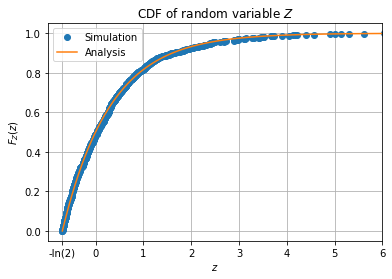
\includegraphics[width=\columnwidth]{solutions/st/2021/19/Figures/CDF_Z.png}
     \caption{$F_Z(z)$}
\end{figure}
Now calculating the expectation value for $Z$, we have
\begin{align}
    E(Z)&=\int\limits_{-\ln{2}}^{\infty}z\,f_Z(z)\,dz\\
    &=\int\limits_{-\ln{2}}^{\infty}\dfrac{z\,e^{-z}}{2}\,dz\\
    &=\left[ \dfrac{-(z+1)\,e^{-z}}{2} \right]_{-\ln{2}}^\infty\\
    &=1-\ln{(2)}\\
    &\approx0.3068
\end{align}


\end{enumerate}